% document formatting
\documentclass[10pt]{article}
\usepackage[utf8]{inputenc}
\usepackage[left=1in,right=1in,top=1in,bottom=1in]{geometry}
\usepackage[T1]{fontenc}
\usepackage{xcolor}

% math symbols, etc.
\usepackage{amsmath, amsfonts, amssymb, amsthm}

% lists
\usepackage{enumerate}

% images
\usepackage{graphicx} % for images
\usepackage{tikz}
\usetikzlibrary{arrows.meta}

% code blocks
% \usepackage{minted, listings} 

% verbatim greek
\usepackage{alphabeta}

\title{Bellman Ford Examples}
 
\author{Aidan Jan}

\begin{document}
\maketitle

\section*{Graph}
https://www.youtube.com/watch?v=obWXjtg0L64
\begin{center}
    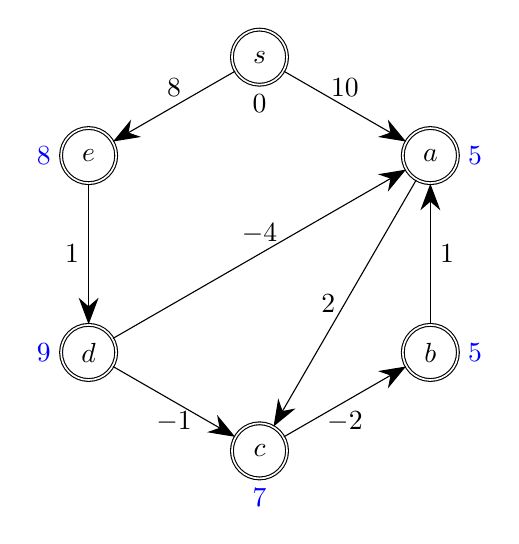
\begin{tikzpicture}
        \node[double, circle, draw, minimum size = 0.7cm, label=below:{\textcolor{black}{$0$}}] at (0, 2.5) (s) {\textcolor{black}{$s$}};
        \node[double, circle, draw, minimum size = 0.7cm, label=right:{\textcolor{blue}{$5$}}] at (2.17, 1.25) (a) {\textcolor{black}{$a$}};
        \node[double, circle, draw, minimum size = 0.7cm, label=right:{\textcolor{blue}{$5$}}] at (2.17, -1.25) (b) {\textcolor{black}{$b$}};
        \node[double, circle, draw, minimum size = 0.7cm, label=below:{\textcolor{blue}{$7$}}] at (0, -2.5) (c) {\textcolor{black}{$c$}};
        \node[double, circle, draw, minimum size = 0.7cm, label=left:{\textcolor{blue}{$9$}}] at (-2.17, -1.25) (d) {\textcolor{black}{$d$}};
        \node[double, circle, draw, minimum size = 0.7cm, label=left:{\textcolor{blue}{$8$}}] at (-2.17, 1.25) (e) {\textcolor{black}{$e$}};

        \draw[-{Stealth[scale=2]}] (s) -- node[above] {$10$} (a);
        \draw[-{Stealth[scale=2]}] (s) -- node[above] {$8$} (e);
        \draw[-{Stealth[scale=2]}] (e) -- node[left] {$1$} (d);
        \draw[-{Stealth[scale=2]}] (d) -- node[below] {$-1$} (c);
        \draw[-{Stealth[scale=2]}] (c) -- node[below] {$-2$} (b);
        \draw[-{Stealth[scale=2]}] (b) -- node[right] {$1$} (a);
        \draw[-{Stealth[scale=2]}] (d) -- node[above] {$-4$} (a);
        \draw[-{Stealth[scale=2]}] (a) -- node[left] {$2$} (c);
    \end{tikzpicture}
\end{center}

\subsection*{Relaxation Queue}
\begin{center}
    \begin{tabular}{c|c|cccccc}
        Step & Queue     & $s$ & $a$ & $b$ & $c$ & $d$ & $e$ \\ \hline
        0 & \texttt{[s]} & $0$ & $\infty$ & $\infty$ & $\infty$ & $\infty$ & $\infty$ \\
        1 & \texttt{[a, e]} & $0$ & $10$ & $\infty$ & $\infty$ & $\infty$ & $8$ \\
        2 & \texttt{[e, c]} & $0$ & $10$ & $\infty$ & $12$ & $\infty$ & $8$ \\
        3 & \texttt{[c, d]} & $0$ & $10$ & $\infty$ & $12$ & $9$ & $8$ \\
        4 & \texttt{[d, b]} & $0$ & $10$ & $10$ & $12$ & $9$ & $8$ \\
        5 & \texttt{[b, a, c]} & $0$ & $5$ & $10$ & $8$ & $9$ & $8$ \\
        6 & \texttt{[a, c]} & $0$ & $5$ & $10$ & $8$ & $9$ & $8$ \\
        7 & \texttt{[c]} & $0$ & $5$ & $10$ & $7$ & $9$ & $8$ \\
        8 & \texttt{[b]} & $0$ & $5$ & $5$ & $7$ & $9$ & $8$ \\
        9 & \texttt{[]} & $0$ & $5$ & $5$ & $7$ & $9$ & $8$ \\
    \end{tabular}
\end{center}

\subsection*{Dynamic Programming}
Recursion:
\[\texttt{OPT}(v, i) = \min \begin{cases}
\texttt{OPT}(v, i - 1) \\
\min_{w \in N(v)} \left[\texttt{OPT}(w, i - 1) + d(w, v)\right]
\end{cases}\]


\end{document}